\begin{enumerate}[label=\thesubsection.\arabic*,ref=\thesubsection.\theenumi,itemsep=1ex]
%\numberwithin{equation}{enumi}
%
\item If $\cos x = -\frac{3}{5}, x$ lies in the third quadrant, find the values of other five trigonometric function.
%
\\
\solution
	In \figref{fig:ncert-id-1}, 
\begin{align}
	a &= -3, b = 5, c = -4
	\\
\implies \cos x &= -\frac{3}{5}\,
\sin x = -\frac{4}{5}\,
\tan x = \frac{-4}{-3}
\end{align}
\begin{figure}[H]
	\begin{center}
		{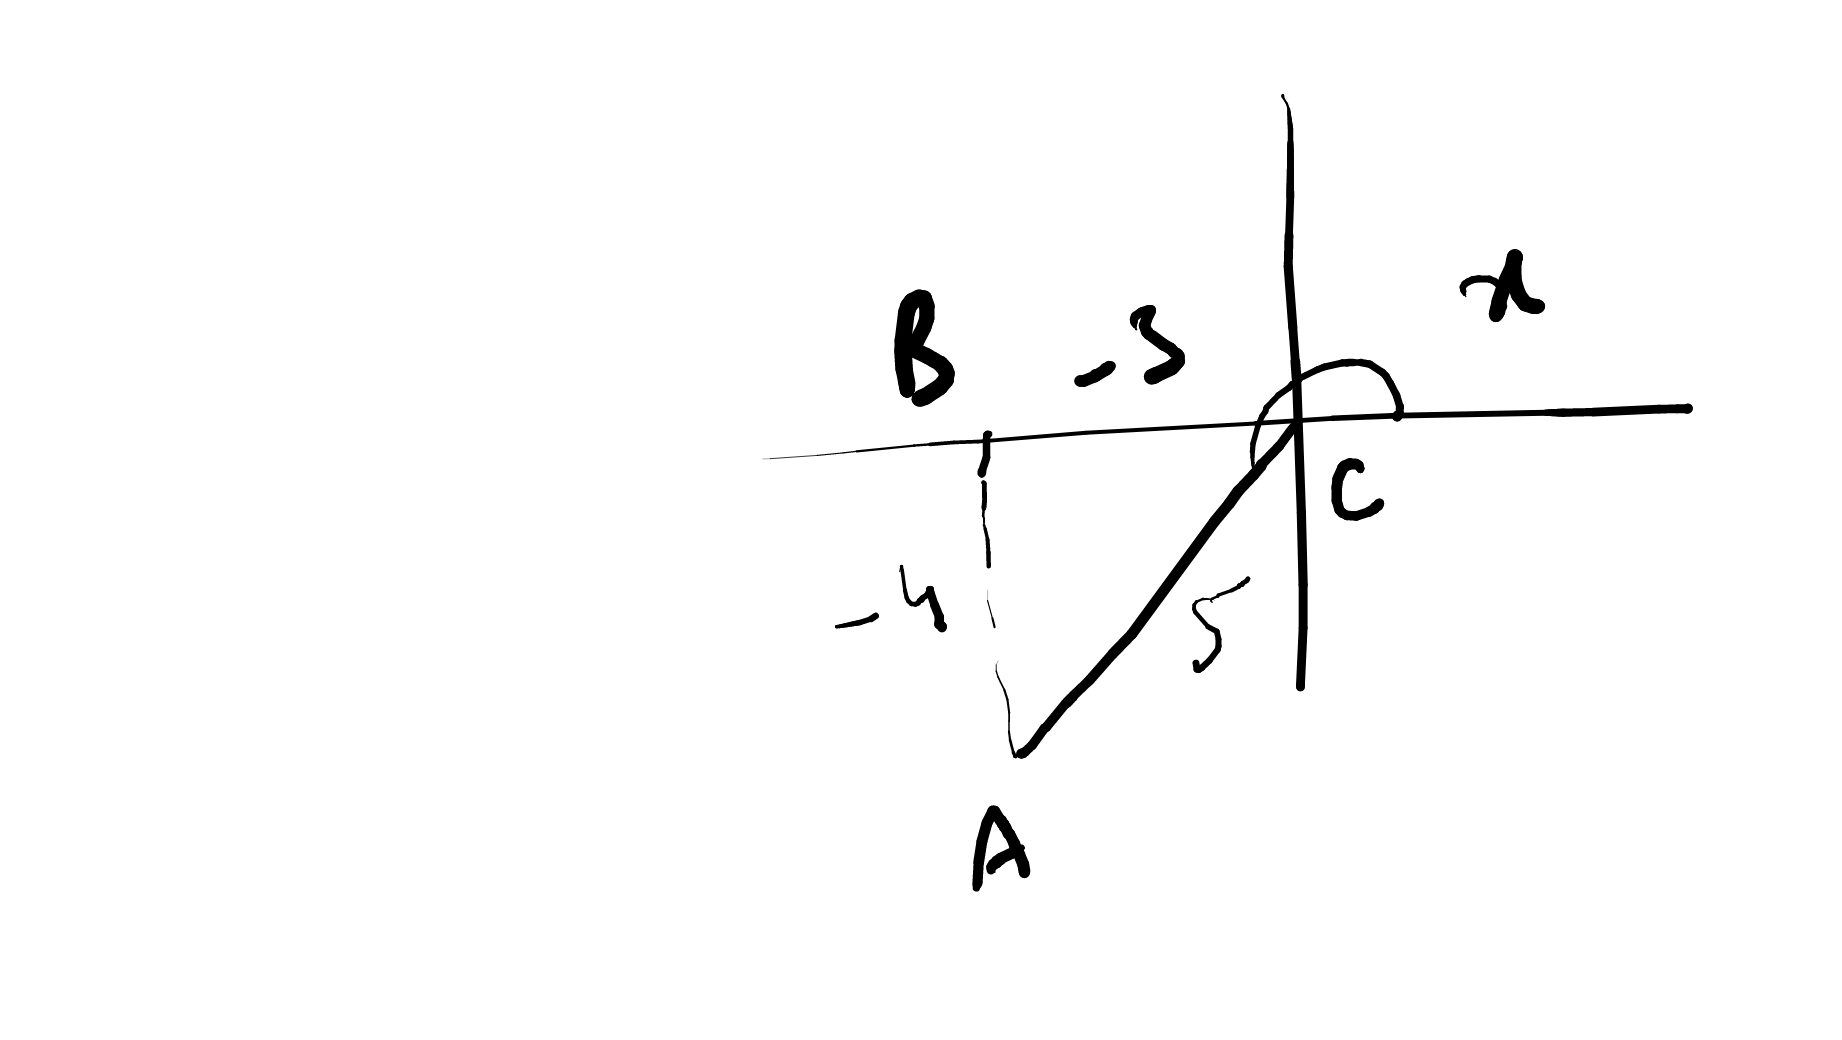
\includegraphics[width=0.6\columnwidth]{figs/ncert/id/1.png}}
	\end{center}
	\caption{}
	\label{fig:ncert-id-1}	
\end{figure}
\item If $\cot x = - \frac{5}{12}, x$ lies in the second quadrant, find the values of other five trigonometric function.
%
\\
\solution
	In \figref{fig:ncert-id-2}, 
\begin{align}
	a &= -5, b = 13, c = 12 
	\\
\implies \cos x &= -\frac{5}{13}\,
\sin x = \frac{12}{13}\,
\tan x = -\frac{12}{5}
\end{align}
\begin{figure}[H]
	\begin{center}
		{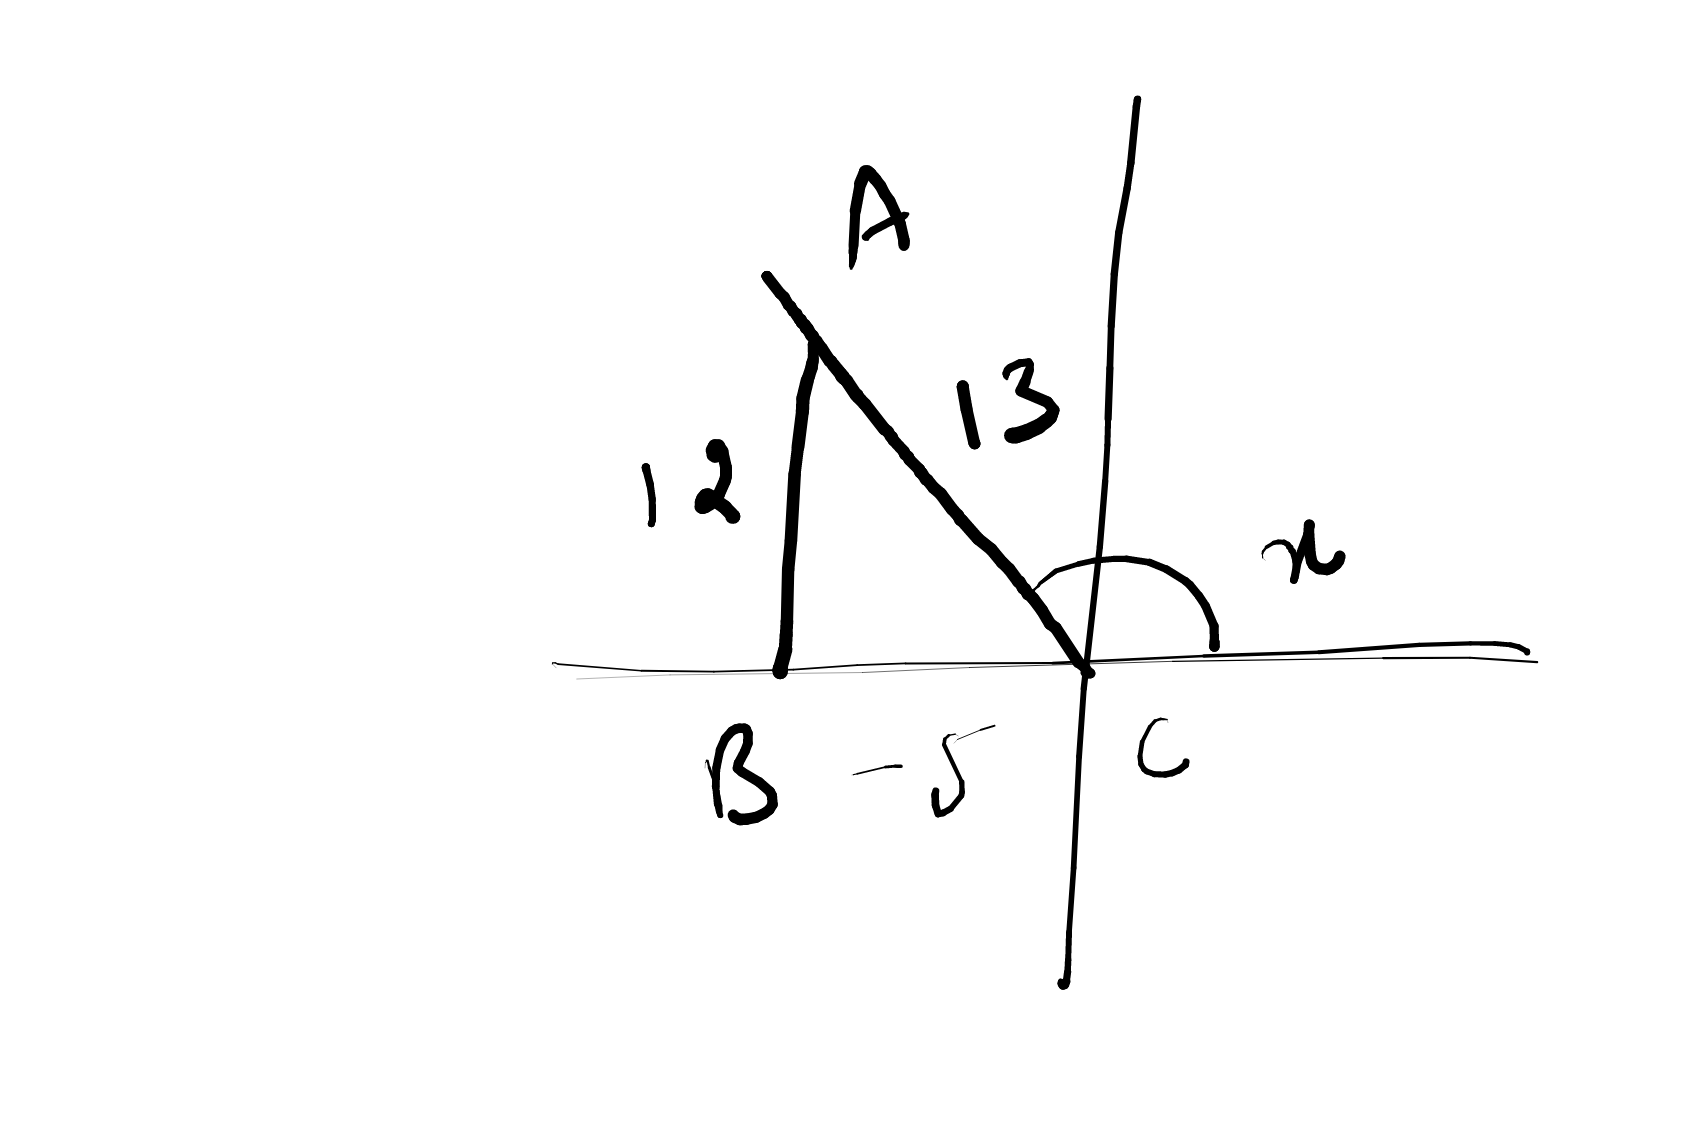
\includegraphics[width=0.6\columnwidth]{figs/ncert/id/2.png}}
	\end{center}
	\caption{}
	\label{fig:ncert-id-2}	
\end{figure}
\item Find the value of $\sin \frac{31\pi}{3}$.
%
	\\
		\solution 
\begin{align}
	\sin \frac{31\pi}{3} &= 
	\sin \brak{10 \pi+\frac{\pi}{3}} 
	\\
	&= 
	\sin \brak{\frac{\pi}{3}} = \frac{1}{2}
\end{align}
\item Find the value of $\cos\brak{-1710\degree}$.
%
	\\
		\solution 
\begin{align}
	\cos\brak{-1710\degree}	&= 
\cos\brak{-5\times360\degree+90\degree}	 
\\
	&=\cos{90\degree}	= 0
\end{align}
\item Prove that $3\sin\frac{\pi}{6}\sec\frac{\pi}{3}-4\sin\frac{5\pi}{6}\cot\frac{\pi}{4} = 1.$
%
	\\
	\solution
\begin{align}
	3\sin\frac{\pi}{6}\sec\frac{\pi}{3}-4\sin\frac{5\pi}{6}\cot\frac{\pi}{4} &= 
	3\frac{\sin\frac{\pi}{6}}{\cos\brak{\frac{\pi}{2}-\frac{\pi}{6}}}-4\sin\brak{\pi - \frac{\pi}{6}}  
	\\
	&=
	3\frac{\sin\frac{\pi}{6}}{\sin\frac{\pi}{6}}-4\sin\brak{ \frac{\pi}{6}}  
	= 1
\end{align}
upon substituting numerical values.
\item Find the value of $\sin 15\degree$.
%
	\\
	\solution 
\begin{align}
	1 - 2 \sin^2 15 &= \cos 30 = \frac{\sqrt{3}}{2}
	\\
	\implies 
	\sin 15 &= \sqrt{\frac{1-\frac{\sqrt{3}}{2}}{2}}
	 = \frac{\sqrt{2-\sqrt{3}}}{2}
	 \label{eq:id-sin15}
\end{align}
\item Find the value of $\tan\frac{13\pi}{12}$.
%
	\\
	\solution 
\begin{align}
\tan\frac{13\pi}{12}
	&=
	\tan\brak{\pi+\frac{\pi}{12}}
=\tan\frac{\pi}{12}
\end{align}
%
Since
\begin{align}
	2 \cos^2 15 -1 &= \cos 30 = \frac{\sqrt{3}}{2},
	\\
	\cos15 &= \sqrt{\frac{1+\frac{\sqrt{3}}{2}}{2}}
	 = \frac{\sqrt{2+\sqrt{3}}}{2}
	 \\
	 \therefore 
	\tan\frac{\pi}{12} &= \frac{\sin 15}{\cos15}
	 = \frac{\sqrt{2-\sqrt{3}}}{\sqrt{2+\sqrt{3}}}
\end{align}
upon substituting from 
	 \eqref{eq:id-sin15}.
\item Prove that $$\frac{\sin\brak{x+y}}{\sin\brak{x-y}} = \frac{\tan x + \tan y}{\tan x - \tan y}.$$
%
%
\item Show that
$\tan3x\tan2x\tan x = \tan3x-\tan2x-\tan x$.
%
%
\item Prove that
$\cos\brak{\frac{\pi}{4}+x} + \cos\brak{\frac{\pi}{4}-x} = \sqrt 2\cos x$.
%
%
\item Prove that $$\frac{\cos7x+\cos5x}{\cos7x-\cos5x} = \cot x.$$
%
%
\item Prove that $$\frac{\sin5x-2\sin3x+\sin x}{\cos5x-\cos x} = \tan x.$$
%
%
\item If $\sin x=\frac{3}{5}, \cos y=-\frac{12}{13}$, where $x$ and $y$
both lies in second quadrant, find the value of
$\sin\brak{x+y}$.
%
%
\item Prove that
$\cos2x\cos\frac{x}{2}-\cos3x\cos\frac{9x}{2}=\sin5x\sin\frac{5x}{2}$.
%
%
\item Find the value of $\tan\frac{\pi}{8}$.
%
%
\item If $\tan x=\frac{3}{4}, \pi<x<\frac{3\pi}{2}$, find the value of $\sin\frac{x}{2},\cos\frac{x}{2}$ and $\tan\frac{x}{2}$.
%
%
\item Prove that
$\cos^{2}x+\cos^{2}\brak{x+\frac{\pi}{3}}+\cos^{2}\brak{x-\frac{\pi}{3}}=\frac{3}{2}$.
%
\item Find the values of other five trigonometric functions 
\begin{enumerate}
	\item $\cos x=-\frac{1}{2}x$,  lies in third quadrant.
	\item $\sin x= \frac{3}{5}x$,  lies in second quadrant.
	\item $\cot x= \frac{3}{4}x$,  lies in third quadrant.
	\item $\sec x= \frac{13}{5}x$,  lies in fourth quadrant.
	\item $\tan x=-\frac{5}{12}x$,  lies in second quadrant.
\end{enumerate}
%
\item Find the values of the trigonometric functions
\begin{multicols}{2}
\begin{enumerate}
\item $\sin765\degree$
\item $\csc\brak{-1410\degree}$
\item $\tan\frac{19\pi}{3}$
\item $\sin\frac{-11\pi}{3}$
\item $\cot\frac{-15\pi}{4}$
\end{enumerate}
\end{multicols}
%
\item Prove that
\begin{multicols}{2}
\begin{enumerate}
\item $\sin^{2}\frac{\pi}{6}+\cos^{2}\frac{\pi}{3}-\tan^{2}\frac{\pi}{4}=-\frac{1}{2}$
\item $2\sin^{2}\frac{\pi}{6}+\csc^{2}\frac{7\pi}{6}\cos^{2}\frac{\pi}{3}=-\frac{3}{2}$
\item $\cot^{2}\frac{\pi}{6}+\csc^{2}\frac{5\pi}{6}+3\tan^{2}\frac{\pi}{6}$=6
\item $2\sin^{2}\frac{3\pi}{4}+2\cos^{2}\frac{\pi}{4}+2\sec^{2}\frac{\pi}{3}$=10
\end{enumerate}
\end{multicols}
%
\item Find the value of
\begin{multicols}{2}
\begin{enumerate}
\item$\sin75\degree$
\item $\tan15\degree$
\end{enumerate}
\end{multicols}
%
\item Prove that 
 $\cos\brak{\frac{\pi}{4}-x}\cos\brak{\frac{\pi}{4}-y}-\sin\brak{\frac{\pi}{4}-x}\sin\brak{\frac{\pi}{4}-y}=\sin\brak{x+y}$.
%
\item Prove that 
$$\frac{\tan\brak{\frac{\pi}{4}+x}}{\tan\brak{\frac{\pi}{4}-x}}=\brak{\frac{1+\tan x}{1-\tan x}}^{2}.$$
%
\item Prove that
$$\frac{\cos\brak{\pi+x}\cos\brak{-x}}{\sin\brak{\pi-x}\cos\brak{\frac{\pi}{2}+x}}=\cot^{2}x.$$
%
\item Prove that
$\cos\brak{\frac{3\pi}{2}+x}\cos\brak{2\pi+x}\sbrak{\cot\brak{\frac{3\pi}{2}-x}+\cot\brak{2\pi +x}}=1$.
%
\item Prove that
$\sin\brak{n+1}x\sin\brak{n+2}x+\cos\brak{n+1}x\cos\brak{n+2}x=\cos x.$
%
\item Prove that
$\cos\brak{\frac{3\pi}{4}+x}-\cos\brak{\frac{3\pi}{4}-x}=-\sqrt 2\sin x.$
%
\item Prove that
$\sin^{2}6x-\sin^{2}4x=\sin2x\sin10x.$
%
\item Prove that
$\cos^{2}2x-\cos^{2}6x=\sin4x\sin8x.$
%
\item Prove that
$\sin2x+2\sin4x+\sin6x=4\cos^{2}x\sin4x.$
%
\item Prove that
$\cot4x\brak{\sin5x+\sin3x}= \cot x\brak{\sin5x-\sin3x}.$
%
\item Prove that
$$\frac{\cos9x-\cos5x}{\sin17x-\sin3x}=-\frac{\sin2x}{\cos10x}.$$
%
\item Prove that
$$\frac{\sin5x+\sin3x}{\cos5x+\cos3x}=\tan4x.$$
%
\item Prove that
$$\frac{\sin x+\sin y}{\cos x+\cos y}=\tan\brak{\frac{x-y}{2}}.$$
%
\item Prove that
$$\frac{\sin x+\sin3x}{\cos x+\cos3x}=\tan2x.$$
%
\item Prove that
$$\frac{\sin x-\sin3x}{\sin^{2}x-\cos^{2}x}=2\sin x.$$
%
\item Prove that
$$\frac{\cos4x+\cos3x+\cos2x}{\sin4x+\sin3x+\sin2x}=\cot3x.$$
%
\item Prove that
$\cot x\cot2x-\cot2x\cot3x-\cot3x\cot x=1$.
%
\item Prove that
$$\tan4x=\frac{4\tan x\brak{1-\tan^{2}x}}{1-6\tan^{2}x+\tan^{4}x}.$$
%
\item Prove that
$\cos4x=1-8\sin^{2}x\cos^{2}x$.
%
\item Prove that
$\cos6x=32\cos^{6}x-48\cos^{4}x+18\cos^{2}x-1$.
%
%
\item Prove that
\begin{enumerate}
\item 2$\cos\frac{\pi}{13}\cos\frac{9\pi}{13}+\cos\frac{3\pi}{13}+\cos\frac{5\pi}{13}=0$
\item $\brak{\sin3x+\sin x}\sin x+\brak{\cos3x-\cos x}\cos x=0$
\item $\brak{\cos x+\cos y}^{2}+\brak{\sin x-\sin y}^{2}=4\cos^{2}\brak{\frac{x+y}{2}}$
\item $\brak{\cos x-\cos y}^{2}+\brak{\sin x-\sin y}^{2}=4\sin^{2}\brak{\frac{x-y}{2}}$
\item $\sin x+\sin3x+\sin5x+\sin7x=4\cos x\cos2x\sin4x$
\item $$\frac{\brak{\sin7x+\sin5x}+\brak{\sin9x+\sin3x}}{\brak{\cos7x+\cos5x}+\brak{\cos9x+\cos3x}}=\tan6x$$
\item $\sin3x+\sin2x-\sin x=4\sin x\cos\frac{x}{2\cos\frac{3x}{2}}$
\end{enumerate}
%
\item Find $\sin\frac{x}{2},\cos\frac{x}{2}$ and $\tan\frac{x}{2}$ in each of the following
\begin{enumerate}
\item $\tan x=-\frac{4}{3}x$,  in second quadrant. 
\item $\sin x=\frac{1}{4}x$,   in second quadrant.
\item $\cos x=-\frac{1}{3}x$,  in third quadrant.
\end{enumerate}
    
\end{enumerate}
    
